
\chapter{Search algorithm}
\label{search_algorithm}



Usually, Lagrangian frameworks involve the computation of the streamlines or projections. The computation of the streamlines is related to the material derivative and is part of the differentiation. The projections are part of the communication between the Lagrangian and Eulerian domains, and belong to the numerical environment. Those task require the search of material points (streamlines) or nodes (projections) over the spatial discretization. This happens both in the fixed mesh PFEM-2 algorithm or in the mesh moving PFEM algorithm. As counterpart to the simplicity in the system computation provided by the Lagrangian algorithms, a search algorithm is required.

In this appendix, the search algorithm used and implemented for the presented work is explained. It is based on the \emph{divide and conquer} strategy. The main domain is firstly partitioned using a dynamic bins structure, a detailed explanation can be found in \textcolor{red}{[............]}. In brief, the dynamic bins are a search structure where the cell size is higher than the characteristic element size. 

\begin{figure}
    \centering
    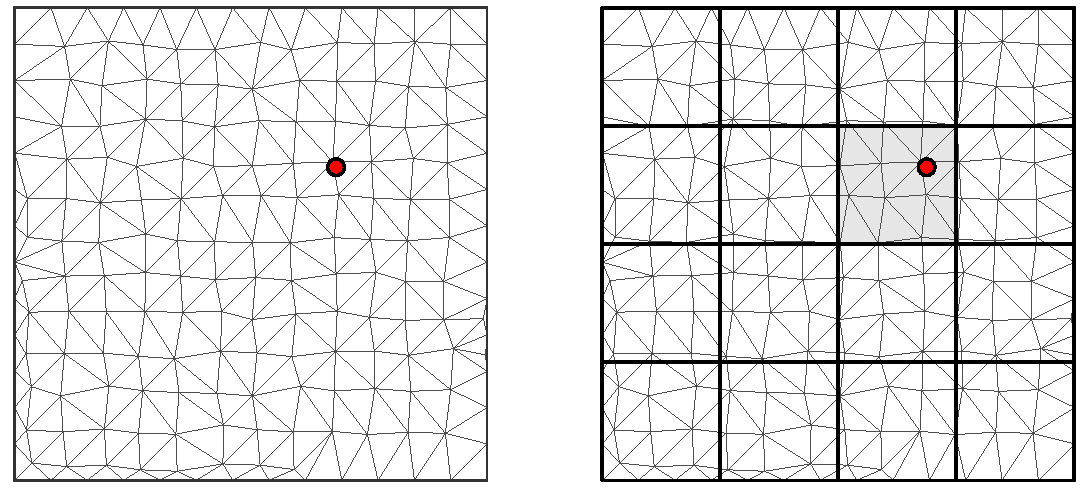
\includegraphics[width=.9\textwidth]{img/search/bins_search.pdf}
    \caption{Left: Mesh and point to locate in the mesh. Right: Mesh and point with the search structure}
    \label{bins_search}
\end{figure}

%El algoritmo de búsqueda se basa en una estructura dinámica bins, explicada con detalle en \textcolor{red}{[............]}. De modo resumico, entre el nodo o entidad a buscar y la malla, se interpone una estructura de búsqueda, que consiste en una partición regular del dominio, definida por un tamaño de celda.

Esta estructura de búsqueda tiene un coste inicial de creación, pero luego, ahorra enormemente el tiempo de búsqueda. En primer lugar, la estructura de búsqueda consiste en la definición de las celdas. En segundo lugar, se realiza una búsqueda entidad a entidad para asociar los elementos intersectados por una celda con ella. La comparación de elementos con celdas podría hacerse mediante proyecciones, sin embargo se ha empleado el método descrito por Möller \cite{moller2004}, que se describe más abajo.

Una vez definida la estructura de búsqueda, el proceso de búsqueda también tiene dos pasos. En primer lugar, se determina en qué celda cae el nodo o partícula en cuestión. Nótese que esta búsqueda es trivial y puede hacerse en paralelo. El resultado será una lista de elementos candidatos. En segundo lugar, se realiza otra búsqueda, más costosa, pero solamente en un número reducido de candidatos. Esta segunda búsqueda requiere hacer una comprobación punto-elemento, que involucra la evaluación de las funciones de forma o bien, el cálculo de proyecciones.



\section{Triangle vs aligned box intersection}

La explicación completa puede encontrarse en \cite{moller2004}. Si bien el problema podría reducirse a un caso 2D, se ha desarrollado la versión genérica 3D, por su extensibilidad a las ecuaciones de convección-difusión, Navier-Stokes u otros problemas. La adaptació al caso bidimensional es trivial y se explicará en este anexo.

La derivación de este algoritmo se basa en el \emph{Separating Axis Theorem} \cite{gottschalk1996}. Consiste en una búsqueda de separating axis entre los dos objetos. La figura \ref{triangle_aabb} muestra los 13 ejes posibles (los tres ejes cartesianos $\mathbf{e}_i$, el vector normal $\mathbf{n}$ y las cominaciones entre los ejes $\mathbf{f}_j$ con $\mathbf{e}_i$). Cuando un test halla un separating axis, el algoritmo de detiene y el resultado es que no hay intersección. Si hay intersección, se ejecutarán todos los test, pues ninguno encontrará un separating axis.

De acuerdo con la Figura \ref{triangle_aabb}, la primera operacion consiste en trasladar el triángulo de modo que el AABB quede centrado en el origen de coordenadas. Los tests a pasar son:

\begin{figure}
\centering
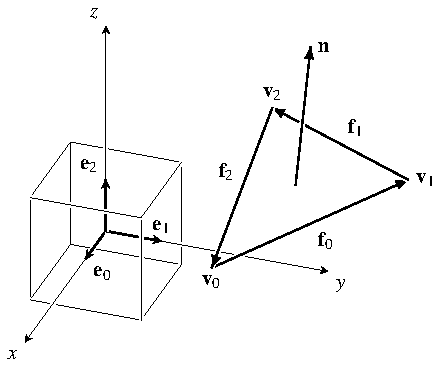
\includegraphics[width=.6\textwidth]{img/search/triangle_aabb.pdf}
\caption{Notación empleada para buscar un separating axis entre triángulo y AABB}
\label{triangle_aabb}
\end{figure}

\begin{description}
    \item[Ejes cartesianos] (3 tests) El primer set de tests consiste en comparar en las tres direcciones $\mathbf{e}_i$ el AABB respecto el mínimo AABB del triángulo. En pseudocódigo la búsqueda de un separating axis queda:
    \begin{verbatim}
for i = 0:2
    min, max = min_max(triangle_points)
    if (min > half_box_size or max < -half_box_size)
        return true
return false
    \end{verbatim} 
    \item[Vector normal] (1 test) El segundo conjunto de tests consiste en una comparación AABB - plano. Para ello se define el plano que contiene el triángulo com el vector normal $\mathbf{n}$ y la distancia a origen $d$. La búsqueda de un separating axis se realiza en el mismo octante que el vector $\mathbf{n}$, de modo análogo al test anterior.
    \item[Aristas] (9 tests) Se realiza un test por cada combinación $\mathbf{a}_{ij} = \mathbf{n}_i \times \mathbf{f}_j$. Cada test supone hacer una proyección del triángulo y el AABB, la comparación se realiza siguiendo el algoritmo del primer test. Afortunadamente, el desarrollo de las proyecciones presenta algunas simplificaciones. Para la primera proyeccion tenemos:
    \begin{align*}
        p_0 &= \mathbf{a}_{00} \cdot \mathbf{v}_0 = (0, -f_{0z}, f_{0,y}) \cdot \mathbf{v}_0 = v_{0z}v_{1y} - v_{0y}v_{1z} \\
        p_1 &= \mathbf{a}_{00} \cdot \mathbf{v}_1 = (0, -f_{0z}, f_{0,y}) \cdot \mathbf{v}_1 = v_{0z}v_{1y} - v_{0y}v_{1z} = p_0 \\
        p_2 &= \mathbf{a}_{00} \cdot \mathbf{v}_2 = (0, -f_{0z}, f_{0,y}) \cdot \mathbf{v}_2 = (v_{1y} - v_{0y}) v_{2z} - (v_{1z} - v_{0z}) v_{2y}
    \end{align*}
    El hecho de que $p_0 = p_1$ facilita la búsqueda del máximo y mínimo de $p_0$, $p_1$ y $p_2$. Éstos se tiene que comparar con el "radio" de la caja, que es la proyección de una esquina sobre $\mathbf{a}_{00}$:
    \begin{align*}
        r = h_x |a_{00x}| + h_y |a_{00y}| + h_z |a_{00z}|
    \end{align*}
    Finalmente, la búsqueda de un separating axis consiste en:
    \begin{verbatim}
        if (min(p0, p2) > r or max(p0, p2) < -r)
            return true
    \end{verbatim}
\end{description}
Si todos los 13 tests descritos devuelven falso, significa que no hay ningún separating axis, e decir, hay intersección entre las dos geometrías. Nótese que solo con que un test de verdadero, el algoritmo se detiene, pues no habrá intersección posible.

\subsection{Particularización para 2D}

El caso bidimensional es una simplificacion del algoritmo general y algunos tests se pueden omitir. En total, se realizan 5 tests:
\begin{description}
    \item[Ejes cartesianos] Se busca un separating axis en $x$ e $y$.
    \item[Vector normal] Se omite.
    \item[Aristas] Solamente son relevantes las proyecciones de las aristas $\mathbf{f}_j$ con el eje $\mathbf{e}_z$.  
\end{description}



\section{Quadrilateral vs aligned box intersection}

El presente algoritmo es fácilmente extrapolable a cuadriláteros. Hay que modificar los tests de las aristas, por un lado, se incluye una arista nueva, por otro lado, cada test requiere de más condicionales, ya que hay un nodo adicional.

Sin embargo, se ha optado por dividir cada cuadrilátero en dos triángulos y realizar dos comprobaciones. Aunque el número de comprobaciones es significativamente mayor, esto supone un ahorro de código y de mantenimiento. El hecho de tomar esta aproximación es que no estamos interesados en la optimización del código, sino en la evaluación del métodos FEM.



\section{Point intersection}

Determinar si un punto está dentro de un triángulo lineal o cuadrilátero bilineal es una operación sencilla. Tan solo es preciso determinar el punto en coordenadas locales y verificar si todas ellas estan entre 0 y 1 en el caso de un triángulo. Entre -1 y 1 en el caso de cuadriláteros. De modo equivalente y para elementos linales o bilineales, esta comprobación se puede expresar en términos de las funciones de forma, permite ahorrar la evaluación de condicionales:
\begin{verbatim}
function is_inside
    for i = 1 : n_nodes
        if N(i) < 0
            return false
    return true
\end{verbatim}



